\section{Measured Baselines}
\label{sec:evidence}
This section establishes three things about the baseline: both coordination boundaries
on the cross-node Direct path carry a cost that does not scale with the payload, that
cost is a large fraction of the operator in the small-batch regime, and the effect
survives in a real serving stack. Everything reported here measures an unmodified
baseline. No in-network prototype exists, and no number in this section is a saving.

\subsection{Setup}
\label{sec:setup}
Measurements come from two H200 nodes, eight GPUs each, connected by
8$\times$400\,GbE RoCE; within each node the GPUs share an NVSwitch fabric. The
transport across nodes is GIN with the GDAKI backend, on traffic class 162. The software stack is
PyTorch 2.13 with CUDA 13, NCCL 2.31.2, and DeepEP at commit
\texttt{01dc3aaa}~\cite{deepepcode}; \emph{Direct} Dispatch and Combine are the
measured path, with Hybrid disabled. Microbenchmarks use $H=7168$, $\topk=8$, 256
experts, BF16, and balanced uniform routing, where $T$ denotes source tokens per rank.

Two conventions govern every number below. First, total operator latency is measured
with tracing off while phase durations are measured with tracing on; the two cannot be
mixed, so a phase duration must never be subtracted from a trace-off total. Second,
each grid point is three independent process runs of 200 active iterations, and the
reported uncertainty is the standard deviation \emph{across runs} rather than across
iterations.

\paragraph{Rank selection.} For each iteration we compute every rank's phase duration,
select the rank whose duration is \emph{shortest}, and divide by that same rank's
traced operator span in the same iteration. Selecting the minimum is deliberate: it
gives the most conservative estimate of coordination cost, since the shortest observed
interval is the one least inflated by waiting on a straggler. The consequence is that
the entry and completion-signal columns may select different ranks, so they
characterize the same configuration but are \emph{not} additive segments of one rank's
time budget. We never sum them.

\subsection{Both boundaries, measured from the same runs}
\label{sec:paired}
Table~\ref{tab:paired} reports the entry and tail windows for EP8 Direct across four
batch sizes. At each $T$ both columns come from the same three instrumented runs and
the same iterations, so they are directly comparable rather than assembled from
separate experiments.

\begin{table}[t]
\centering\small
\setlength{\tabcolsep}{4pt}
\begin{tabular}{llrr}
\toprule
$T$/rank & Operator & Entry sync & Signal window\\
\midrule
8 & Dispatch & 20.57\%\,$\pm$\,0.06 & 19.33\%\,$\pm$\,0.19\\
  &          & (15.09\,$\pm$\,0.06\us{}) & (14.26\,$\pm$\,0.16\us{})\\
8 & Combine  & 19.84\%\,$\pm$\,0.13 & 17.66\%\,$\pm$\,0.57\\
  &          & (15.15\,$\pm$\,0.03\us{}) & (13.49\,$\pm$\,0.35\us{})\\
\midrule
32 & Dispatch & 12.25\%\,$\pm$\,0.17 & 9.50\%\,$\pm$\,0.40\\
   &          & (15.35\,$\pm$\,0.46\us{}) & (11.61\,$\pm$\,0.30\us{})\\
32 & Combine  & 12.26\%\,$\pm$\,0.26 & 9.38\%\,$\pm$\,0.50\\
   &          & (15.04\,$\pm$\,0.22\us{}) & (11.32\,$\pm$\,0.46\us{})\\
\midrule
64 & Dispatch & 8.29\%\,$\pm$\,0.51 & 6.31\%\,$\pm$\,0.84\\
   &          & (14.90\,$\pm$\,0.10\us{}) & (11.19\,$\pm$\,0.84\us{})\\
64 & Combine  & 8.20\%\,$\pm$\,0.16 & 6.45\%\,$\pm$\,0.16\\
   &          & (14.82\,$\pm$\,0.13\us{}) & (11.57\,$\pm$\,0.23\us{})\\
\midrule
128 & Dispatch & 4.88\%\,$\pm$\,0.04 & 3.79\%\,$\pm$\,0.10\\
    &          & (15.05\,$\pm$\,0.21\us{}) & (11.63\,$\pm$\,0.38\us{})\\
128 & Combine  & 5.05\%\,$\pm$\,0.19 & 3.95\%\,$\pm$\,0.35\\
    &          & (14.95\,$\pm$\,0.23\us{}) & (11.61\,$\pm$\,0.70\us{})\\
\bottomrule
\end{tabular}
\caption{H200 two-node EP8 Direct. Shares are of the selected rank's traced operator
span; uncertainties on shares are in percentage points. Each column selects its own
rank-minimum, so the two are not additive. $T=8$/128 and $T=32$/64 were acquired in
separate sessions on the same instrumented image.}
\label{tab:paired}
\end{table}

The absolute durations are the point. Across a sixteen-fold range in $T$, entry
synchronization stays within 14.8--15.4\us{} for both operators with no trend, and the
signal window settles at 11.2--11.6\us{} once $T \geq 32$. The shares meanwhile fall
monotonically by roughly a factor of four, from about 20\% to about 5\%. Four batch
sizes rather than two matter here: two endpoints alone would be equally consistent with
a coordination cost that shrinks gradually as the batch grows, whereas the intermediate
points show the shares collapsing while the underlying durations stay flat. This is the
signature of a fixed cost, negligible at large batches and dominant at small ones, and
its share is a statement about the denominator rather than about the coordination
itself. One caveat on reading the tail column too finely: the $T=64$ Dispatch signal
window has a between-run deviation of 0.84\us{}, so we do not claim a strict ordering
of absolute signal durations in $T$.

\paragraph{What the tail window is, and is not.} Defining the tail window correctly
required a boundary audit, whose result constrains how it may be read. The enclosing
tail-barrier call is \emph{not} usable as a synchronization measurement: its start can
precede the first remote payload injection, so the envelope covers ongoing data work,
TMA waits, and GIN flush in addition to control. In one instrumented Dispatch
iteration the tail region began 19.97\us{} after kernel entry while the first remote
payload was not issued until 21.66\us{}, and the region did not end until 456.99\us{};
the signal exchange inside it accounted for roughly 15\us{}. We therefore report only
the inner window, from first signal initiation to observation of all expected signals.
Even this narrower window includes GPU-side initiation, polling, and any wait for a
peer that is not yet ready, so it bounds the pure control traversal from above and is
not a bare network RTT.

\subsection{Fixed entry cost, growing tail envelope}
\label{sec:fits}
Fitting the same rank-minimum durations across EP sizes separates the two boundaries
cleanly. Entry synchronization is well described by a constant $a$, whereas the tail
envelope requires $b + cT$ (Table~\ref{tab:fits}). We fit on $T \in \{8, 32, 128\}$ and
hold out $T=96$ as an independent check, without refitting after seeing it. The $T=64$
measurements of Table~\ref{tab:paired} were acquired later and are not part of this fit
or its hold-out.

\begin{table}[t]
\centering\small
\setlength{\tabcolsep}{3.5pt}
\begin{tabular}{lrrll}
\toprule
EP & \multicolumn{2}{c}{Entry sync (\us{})} & \multicolumn{2}{c}{Tail envelope (\us{})}\\
 & Disp. & Comb. & Dispatch & Combine\\
\midrule
4  & 11.64 & 11.54 & $40.87 + 0.546T$ & $33.37 + 0.613T$\\
8  & 15.01 & 14.99 & $37.00 + 1.900T$ & $31.14 + 1.846T$\\
16 & 18.39 & 18.30 & $37.78 + 2.731T$ & $31.97 + 2.424T$\\
\bottomrule
\end{tabular}
\caption{Local empirical fits for H200 cross-node Direct, valid for $T=8$--128.
Maximum held-out error at $T=96$ is 0.96\% for entry synchronization and 4.39\% for the
tail envelope. EP sizes are fitted separately and are categorical: these are not
rank-scaling laws. The tail envelope includes data drain and local join, so it is not a
pure post-synchronization cost.}
\label{tab:fits}
\end{table}

\begin{figure*}[t]
\centering
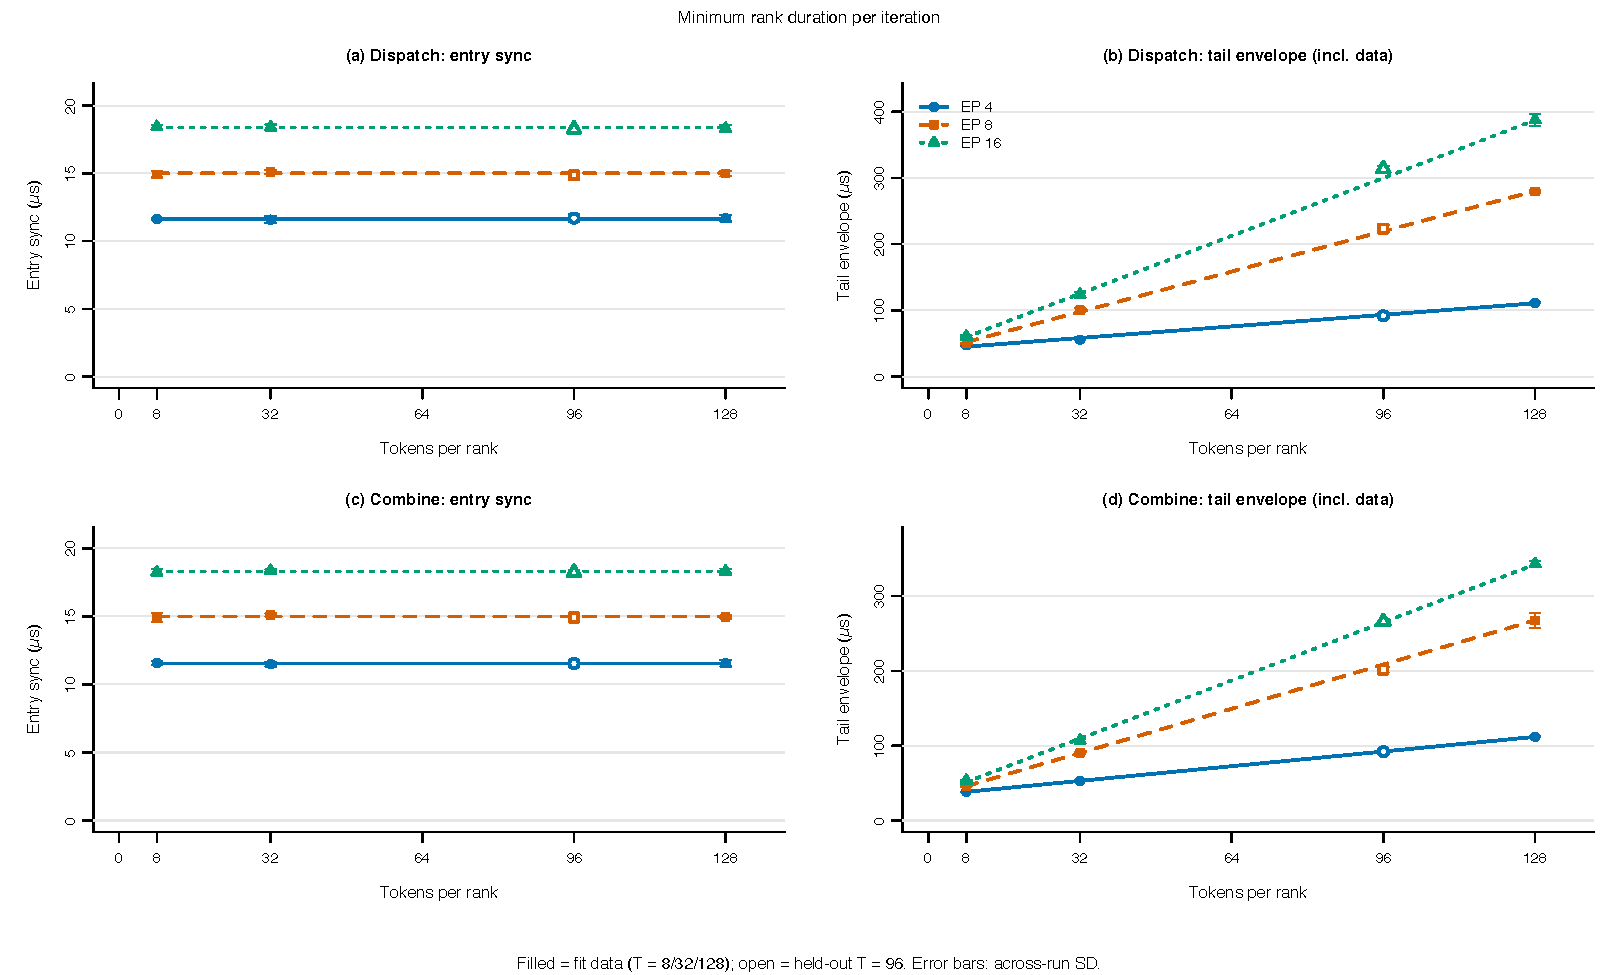
\includegraphics[width=0.92\textwidth]{figures/h200_direct_sync_min_fit.pdf}
\caption{Rank-minimum entry coordination and tail envelope against tokens per rank.
Filled points are the fitted $T \in \{8,32,128\}$; open points are the held-out
$T=96$. Error bars are the standard deviation across runs. Entry coordination is flat
in $T$ at every EP size. The right-hand column includes data-completion waiting and
must not be read as pure post-synchronization.}
\label{fig:fits}
\end{figure*}

Entry synchronization is flat in $T$ and rises with EP size, from roughly 11.6\us at
EP4 to 18.4\us{} at EP16, the behavior expected of a group-wide announcement rather
than a data-dependent transfer. The tail column behaves differently, and its slope is
precisely why we decline to treat it as synchronization: a term proportional to $T$ is
a data term. We report the envelope for completeness and draw tail conclusions only
from the narrow signal window of \secref{sec:paired}. Taking the rank-minimum does not
repair this, because the envelope's boundary problem is internal to each rank. Larger
$T$ also develops a congestion tail, so we do not extrapolate these lines.

\subsection{The effect survives in a serving stack}
\label{sec:e2e}
Balanced-routing microbenchmarks could in principle overstate the effect, so we also
measure Qwen3-30B-A3B (BF16, $H=2048$, 128 experts) under vLLM 0.27 with DeepEP V2
Direct and real model routing. Holding EP8 and decode with 128 input and 128 output
tokens fixed, we vary only the topology (Table~\ref{tab:e2e}).

\begin{table}[t]
\centering\small
\setlength{\tabcolsep}{5pt}
\begin{tabular}{llrr}
\toprule
Topology & Conc. & $T$/rank & Entry sync of GPU step\\
\midrule
1 node, 8 ranks & 64  & 8  & 9.33\%\,$\pm$\,0.12\\
2 nodes, 4 each & 64  & 8  & 16.72\%\,$\pm$\,0.10\\
1 node, 8 ranks & 128 & 16 & 7.94\%\,$\pm$\,0.15\\
2 nodes, 4 each & 128 & 16 & 15.19\%\,$\pm$\,0.05\\
\bottomrule
\end{tabular}
\caption{Qwen3-30B-A3B decode at fixed EP8. Shares pair each rank's Dispatch and
Combine entry synchronization with its own GPU step, averaged over ranks and three
client windows. Crossing the node boundary roughly doubles the share at equal EP size
and concurrency.}
\label{tab:e2e}
\end{table}

At equal EP size and concurrency, crossing the node boundary roughly doubles the
entry-synchronization share, from 8--9\% to 15--17\%. Three caveats bound this result.
The share is of GPU step time, not of request latency, and is therefore not a bound on
any end-to-end speedup. The three repetitions are client windows against one server
instance, not three independent restarts. And the model's $H$ and expert count differ
from the microbenchmark, so absolute durations from Tables~\ref{tab:paired}
and~\ref{tab:e2e} cannot be composed. We report only the entry component here: the
narrow completion-signal window was not instrumented per layer in this campaign, so the
corresponding tail share in a real model remains unmeasured.

\subsection{Sensitivity of the analytical opportunity}
\label{sec:sensitivity}
\begin{figure}[t]
\centering
\begin{tikzpicture}
\begin{axis}[width=\columnwidth,height=4.8cm,
 xlabel={Added overhead $\epsilon_k/L$},ylabel={Net saving $\Delta T_k/L$},
 xmin=0,xmax=2.5,ymin=-1.5,ymax=2.15,
 xtick={0,.5,1,1.5,2,2.5},ytick={-1,0,1,2},
 tick label style={font=\footnotesize},label style={font=\footnotesize},
 legend style={font=\footnotesize,at={(.98,.98)},anchor=north east,draw=none,fill=white},
 grid=major,grid style={black!10},axis lines=left]
\addplot[black!50,thin,domain=0:2.5,forget plot] {0};
\addplot[datablue,thick,domain=0:2.5] {2-x};
\addlegendentry{Two eligible boundaries}
\addplot[controlorange,thick,dashed,domain=0:2.5] {1-x};
\addlegendentry{One eligible boundary}
\end{axis}
\end{tikzpicture}
\caption{Analytical sensitivity of net saving $kL-\epsilon_k$ to added overhead. Under the reference assumptions, the break-even overhead is $L$ for one eligible boundary and $2L$ for two.}
\label{fig:analytical}
\Description{Two analytical lines show normalized saving declining with added overhead. The one-boundary line crosses zero at one unit of one-way delay; the two-boundary line crosses at two.}
\end{figure}

Figure~\ref{fig:analytical} evaluates Equation~\eqref{eq:eligible} with normalized
parameters, sweeping added overhead against one-way propagation. With one eligible
boundary the net saving reaches zero at $\epsilon_1 = L$; with two, at
$\epsilon_2 = 2L$. The curves show how much overhead the design can absorb before the
opportunity disappears, which is the question an implementation actually faces. They
are not a predicted speedup: $\epsilon$ is swept independently rather than fitted to
any measurement.

Converting a measured share into a speedup is tempting, and we want to be explicit
about why we do not. A 20\% entry-synchronization share corresponds to a
$1/(1-0.2) = 1.25\times$ component-removal reference only if that component were
removed entirely at an otherwise identical operating point. Retained local
dependencies, notification overhead, and changed queuing all reduce the removable
portion. A measured 15\us{} entry window also contains endpoint work and is not a
measurement of $L$, so it cannot be substituted into the model as one.

\subsection{Limitations}
\label{sec:limits-evidence}
The evidence is baseline measurement only. Microbenchmarks use balanced uniform routing
and do not characterize real-serving readiness skew; the serving measurements supply
real routing but only for the entry component. We have not measured the quantities that
would pin down the achievable tail saving: sender completion $c_j$, destination
visibility $\tau_d$, and signal-based release $z_d$ from \secref{sec:directtail} as
three distinct observations on one cross-node Direct configuration. Last PUT issuance,
kernel exit, and flush return are all poor substitutes for destination visibility, and
the GIN flush contract explicitly does not promise it. There is no in-network hardware
in this study, so neither the added overhead $\epsilon$ nor any end-to-end effect is
measured, and the analytical curves cannot establish a serving speedup or a
non-regression guarantee.
